\section{Problem statement}
\label{sec:problem}

\cheng{Move this to paragraph, and figure, to Section 2. You need to discuss the problem we are solving before you can talk about related work.}

Suppose we have a dataset $\DCal$ with $N$ playlists from $U$ users, songs in every playlist are from a music collection
with $M$ songs, and each song in the collection is appeared in at least one playlist.

The task of recommending a set of songs to form a playlist for a given user is illustrated in Figure~\ref{fig:gen},
where rows represent songs (no specific order) and columns represent playlists (no specific order).
Further, columns with white colour represent playlists in training set,
and columns with grey colour represent playlists in test set.
If entry $(m, i)$ is \texttt{1} (or \texttt{0}),
it means song $m$ can (or not) be found in playlist $i$,
and a question mark \texttt{?} means we do not know whether song $m$ is in playlist $i$.
As a remark, columns represent playlists in test set contain only \texttt{?} entries.

%\begin{figure}[h]
%\centering
%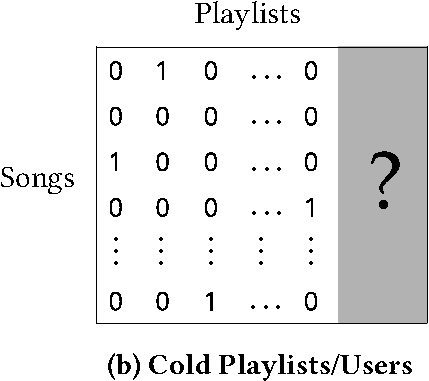
\includegraphics[width=.5\linewidth]{fig/fig_gen.pdf}
%\caption{Illustration of music recommendation setting.}
%\label{fig:gen}
%\end{figure}

% playlists are organised by users. j \in P_i, i \in {1,...U}

\cheng{Update Figure 1 to include meaning of rows and columns. Why do we bother with ?, since the whole test set is unknown? Indicate the effect of known and unknown users.}

\cheng{In 2-3 sentences, define the problem we are attacking in this paper. Recommend a set, not a single item. User specific. All songs known. Consider cold start user.}

\cheng{This should be followed by related work, where you need to describe for each group how we are different, or how we use some idea.}


We aim to learn a function $f(m, n)$ that measure the affinity between song $m$ and playlist $n$,
suppose $f(m, n)$ has a linear form
$$
f(m, n) = \w_n^\top \x_m, \ m \in \{1,\dots,M\}, \, n \in \{1,\dots,N\},
$$
where vector $\w_n$ represents the parameters of playlist $n$ and $\x_m$ is a feature vector of song $m$.


